%%---------------------------------------------------------------------------%%
%% draco-release.tex
%% CCS-2 Draco Team.
%% $Id$
%%---------------------------------------------------------------------------%%
%\documentclass[11pt]{nmemo}
\documentclass[note]{newmemo}
\usepackage[centertags]{amsmath}
\usepackage{amssymb,amsthm,graphicx}
%\usepackage[mathcal]{euscript}
%\usepackage{tmadd,tmath}
\usepackage{tabularx}
\usepackage{cite}
\usepackage{c++}
\usepackage{listings}
\usepackage{color}
\usepackage[colorlinks]{hyperref}

%%---------------------------------------------------------------------------%%
%% DEFINE SPECIFIC ENVIRONMENTS HERE
%%---------------------------------------------------------------------------%%
%\newcommand{\elfit}{\ensuremath{\operatorname{Im}(-1/\epsilon(\vq,\omega)}}
%\msection{}-->section commands
%\tradem{}  -->add TM subscript to entry
%\ucatm{}   -->add trademark footnote about entry


\newcolumntype{L}{>{\ttfamily}X}
\newcommand{\tableText}[1]{{\raggedright #1}}

\newcommand{\draco}{{\normalfont\small\sffamily Draco}}
\newcommand{\jayenne}{{\normalfont\small\sffamily Jayenne}}
\newcommand{\milagro}{{\normalfont\small\sffamily Milagro}}
\newcommand{\capsaicin}{{\normalfont\small\sffamily Capsaicin}}
\newcommand{\wedgehog}{{\normalfont\small\sffamily Wedgehog}}
\newcommand{\clubimc}{{\normalfont\small\sffamily ClubIMC}}

\newcommand{\dox}{\textsf{Doxygen}}
\newcommand{\cmake}{\textsf{CMake}}
\newcommand{\ctest}{\textsf{CTest}}
\newcommand{\cdash}{\textsf{CDash}}
\newcommand{\scons}{\textsf{SCons}}
\newcommand{\cvs}{\textsf{CVS}}  
\newcommand{\valgrind}{\textsf{valgrind}}  
\newcommand{\make}{\textsf{Make}}
\newcommand{\gpp}{\textsf{g++}}

\newcommand{\defect}[1]{{\href{https://tf.lanl.gov/sf/sfmain/do/go/#1}{#1}}}

\definecolor{listingBG}{rgb}{0.95,0.95,0.95}

%% \lstset{language=C++,
%%         showstringspaces=false,
%%         frame=shadowbox,
%%         basicstyle=\footnotesize,
%%         rulesepcolor=\color{black},
%%         backgroundcolor=\color{listingBG}}

\hypersetup{
    %bookmarks=true,         % show bookmarks bar?
    %bookmarksopen=true,     % show the bookmarks bar
    unicode=false,          % non-Latin characters in Acrobat’s bookmarks
    pdftoolbar=true,        % show Acrobat’s toolbar?
    pdfmenubar=true,        % show Acrobat’s menu?
    pdffitwindow=false,     % window fit to page when opened
    %pdfstartview={FitH},    % fits the width of the page to the window
    %pdftitle={My title},    % title
    %pdfauthor={Author},     % author
    %pdfsubject={Subject},   % subject of the document
    %pdfcreator={Creator},   % creator of the document
    %pdfproducer={Producer}, % producer of the document
    %pdfkeywords={keyword1} {key2} {key3}, % list of keywords
    pdfnewwindow=true,      % links in new window
    colorlinks=false,       % false: boxed links; true: colored links
    linkcolor=cyan,         % color of internal links
    citecolor=green,        % color of links to bibliography
    filecolor=magenta,      % color of file links
    urlcolor=blue           % color of external links
}

%%---------------------------------------------------------------------------%%
%% BEGIN DOCUMENT
%%---------------------------------------------------------------------------%%
\begin{document}

%%---------------------------------------------------------------------------%%
%% OPTIONS FOR NOTE
%%---------------------------------------------------------------------------%%

\toms{Distribution}
%\toms{Joe Sixpak/XTM, MS B226}
\refno{CCS--2:12-04(U)}
\subject{Draco Release Policy and Procedures}

%-------NO CHANGES
% orig 
% \divisionname{Applied Theoretical \& Computational Physics Div.}
%\groupname{X-TM:Transport Methods Group}

%\divisionname{Computer and Computational Sciences}
\groupname{CCS--2: Computational Physics \& Methods}
\groupmail{CCS-2, Mail Stop D413}
\groupphone{Phone: 505-667-7029 Fax: 505-665-4972}
\fromms{
   Kelly Thompson/CCS--2, D409
%   Thomas M. Evans \vspace{0.4 em}
}
\phone{(505)665--8090}
\originator{kgt}
\typist{kgt}
% revision 1 \date{May 26, 1999}
% revision 3 
\date{Jan 24, 2012}
%-------NO CHANGES

%-------OPTIONS
%\reference{NPB Star Reimbursable Project}
%\thru{P. D. Soran, XTM, MS B226}
%\enc{list}      
%\attachments{list}
%\cy{list}
%\encas
%\attachmentas
%\attachmentsas 
%-------OPTIONS

%%---------------------------------------------------------------------------%%
%% DISTRIBUTION LIST
%%---------------------------------------------------------------------------%%

\distribution {
Baker Randal S.           CCS-2      D409  \\
Budge Kent G.             CCS-2      D409 \\
Chang Jae Ho              CCS-2      D409 \\
Densmore Jeffery D.       CCS-2      D409 \\
Lowrie Robert B.          CCS-2      D413\\
Palmer Todd S.            CCS-2      D409 \\
Rockefeller Gabriel M.    CCS-2      D409 \\
Rosa Massimiliano         CCS-2      K784 \\
Turner Scott A.           CCS-2      D409\\
Urbatsch Todd J.          CCS-2      D409 \\
Warsa James S.            CCS-2      D409\\
Wollaber Allan B.         CCS-2      D409\\
\\
CCS--2 Files D409 \\
}

%%---------------------------------------------------------------------------%%
%% BEGIN NOTE
%%---------------------------------------------------------------------------%%

\opening

\begin{abstract}

The purpose of this memo is to outline the release policy and
procedures for \draco.  This document is derived from the original
memorandum written in 1999 by Tom Evans~\cite{xtm:9936} and shares
many features with the FreeBSD Release Engineering
process~\cite{freebsd-release-eng}.  These procedures should also
apply to \draco-clients such as \capsaicin\footnote{Email Jae Chang
  (jhchang@lanl.gov) for details}, and \jayenne\ (\clubimc, \wedgehog,
\milagro)\footnote{Email Todd Urbatsch (tmonster@lanl.gov) for
  details}.  We require releases in order to provide capability to
users and for developers of software products that use \draco's
capabilities.  Formal releases allow CCS--2 code projects to maintain
quality control, code reference, and project planning sanity. They are
also used to provide usability, capability and performance
enhancements.

This memo contains two primary sections. Section~\ref{sec:policy}
covers release policy and \S~\ref{sec:procedures} reviews the
mechanics used to produce a release.  An Overview
(\S~\ref{sec:overview}) and Summary (\S~\ref{sec:summary}) are also
provided.

\end{abstract}

%%---------------------------------------------------------------------------%%

\section{Overview}
\label{sec:overview}

\draco\ evolved as a loose collection of individual components bound
by a common build-system.  While \draco\ is more tightly integrated in
its present incarnation, \draco\ development still concentrates on
individual components.  \draco\ components are written in C++, utilize
an Object Oriented Design (OOD), enforce Design-by-Contract
verification, enforces component level encapsualtion and levelized
dependency between components.  \draco\ is a software project that is
continually evolving.  Many components that were once actively
developed and used have been retired to the \cvs\ Attic.  New
components are frequently added to meet today's programming
requirements.

Historically, the general release policy in \draco\ is to separate the
package release number (e.g.: \texttt{c4-3\_1\_0}) from the
\draco\ release number (e.g.: \texttt{draco-6\_3\_0}).  Today,
\draco\ component numbers are fully synchronized with the
\draco\ release number.  This change was made because \draco\ is
relatively small and tagging of individual components wasn't usually
necessary.

The next section (\S~\ref{sec:nomenclature}) of this document covers
some nomenclature followed by a description of the \draco\ release
policy.  Adherence to these policies will expedite code reviews in the
\draco\ project and will present a clean interface to outside users.
Deviations from policies described herein are allowed under special
circumstances as judged by the \draco\ project team.  The
\draco\ release procedure as descirbed in \S~\ref{sec:procedures}
utilizes the \cvs\ version control system.  Thus, \draco\ developers
should peruse the \cvs\ manual~\cite{cvs} to become intimate with its
controls and use.

\section{Nomenclature}
\label{sec:nomenclature}

At this point, we will illuminate some terminology that will be used
throughout this memorandum.  In the \draco\ source directory tree, any
grouping of files that shares a common purpose is a \draco\ {\it
  component}.  Examples of \draco\ {\it components} are
\texttt{draco/src/c4/} and \texttt{draco/config/}. {\it
  \draco-clients} are code systems that use \draco\ components.
\capsaicin\ and \milagro\ are {\it \draco-clients}.  \draco\ {\it
  products} refer to anything produced from the \draco\ source-code
tree (e.g. \texttt{librtt\_c4.so}).  On a final note, the term {\it
  packages} is often used in a supra-\draco\ sense.  \milagro\ and
\capsaicin\ are referred to as {\it packages}.  These are
fundamentally different than \draco\ packages.  While we try to keep
these distinctions firmly in place, one must often derive the meaning
of package from context.


%%---------------------------------------------------------------------------%%
 
\section{Draco Release Policies}
\label{sec:policy}

The \draco\ release policy is a set of general requirements that
controls the process of software release in the \draco\ code system.
To start, we will write down the software release policies for \draco.
Afterwards, we describe these policies in more detail.  Note that
these policies may be waived in special circumstances by the
\draco\ development team.

The \draco\ release policies are:
\begin{enumerate}
\item Agreement to release: The \draco\ board must agree to the
  release content, schedule and determine if the release will be
  considered a major or minor release.
\item All components must pass their respective suite of regression
  tests on all target platforms.  Inspection of the
  \href{http://coder.lanl.gov/cdash}{project dashboard} is sufficient
  for this check.
\item Each \draco\ component must compile without error or warning
  using the build system standard compile flags.  For this test, the
  code be configured, built and testing in at least two
  configurations:
  \begin{enumerate}
  \item Debug: 
    \texttt{-DCMAKE\_BUILD\_TYPE=DEBUG} 
    \texttt{-DGCC\_ENABLE\_ALL\_WARNINGS=ON} 
    \texttt{-DGCC\_ENABLE\_GLIBCXX\_DEBUG=ON} 
  \item Release: 
    \texttt{-DCMAKE\_BUILD\_TYPE=RELEASE}
  \end{enumerate}
  For each of these build types, all warnings should be eliminated
  before the release.  Inspection of the
  \href{http://coder.lanl.gov/cdash}{project dashboard} is sufficient
  is sufficient for this check.
\item The release sponsor must update the \texttt{ChangeLog} to
  reflect items to be included in the release.  Then the \draco\ board
  will review the changes, assign and release number and set a target
  release date. A notification of the intended release will be emailed
  to the \draco\ mailing list (\url{draco@lanl.gov}).  The
  \texttt{ChangeLog} entry for the release must include the following
  information:
  \begin{enumerate}
    \item The tag name (release revision name) must conform to
      requirements listed in \S~\ref{sec:rel_num}.
    \item Associated client-software release names.
    \item Target platforms and compilers for the release.
%    \item Associated vendor libraries must be identified by version
%    and location.
    \item Executive summary of changes included with the release.
    \item A detailed description of changes implemented for each
      component (including changes build system and the developer
      environment). 
    \item A list of known defects.
    \item A list of defects resolved in this release.
    \item Code metrics including lines-of-code and code coverage
      values.
  \end{enumerate}

\item \draco\ must pass a review that validates the release.  The
  review team will include, at a minimum, all \draco\ developers that
  have contributed to any components since the last \draco\ release.
  Any objections concerning the release content or schedule from
  \draco\ team members must be communicated through the
  \draco\ mailing list.  Objections might call out scheduling issues
  or major defects that must be resolved before the release can
  continue.

\item For major relases, a release memorandum must be generated by the
  sponsor that includes all of the \texttt{ChangeLog} information.
  The memorandum must include the following information:
  \begin{enumerate}
    \item All of the items from the \texttt{ChangeLog} as listed above.
    \item A list of contributing authors.
    \item A brief history of prior releases (see
      \S~\ref{sec:author_list}).
    \item A brief discription of each component provided in the
      release. 
    \item A discussion of design requirements: levelized component
      dependencies, thorough Design-by-Contract, unit testing,
      inheritance, etc.
    \item A figure showing the levelized component dependencies.
    \item A plot showing the lines-of-code evolved through time.
    \item Details about installation location and build options.
    \item A quick start guide for \draco\ developers and for
      developers who will use files from a \draco\ installation.
  \end{enumerate}
\item Each file in \draco\ will have at least a \draco-level tag
  conforming to the requirements listed in \S~\ref{sec:rel_num}.  The
  \draco\ tag is a numbered release tag that refers to a fully-stable,
  released version of \draco. Additional \draco\ components such as
  \texttt{doc/}, ~\texttt{config/}, ~\texttt{environment/} and
  ~\texttt{autodoc/} may or may not have tags in addition to the
  common tags.  This is a discretionary policy of the \draco\ team.

\item Each component must have its own unit tests that cover 70\% of
  the component code base as measured by the nightly code coverage
  testing scripts (Bullseye Code Coverage\cite{bullseyeweb} reported
  on the CCS--2 developer's dashboard\cite{codercdash,cmake}.

\item Any priority 1 defects listed in the \draco\ bug tracker
  (\href{https://tf.lanl.gov/sf/tracker/do/listTrackers/projects.draco/tracker}{TeamForge})
  must be closed. 

\item The major numbers on \draco\ numbered release tags should
  correspond to the \cvs\ revision numbers.

\item No non-\draco\ tags should exist in \draco\ components that sit
  under the \texttt{draco/} directory in \texttt{\$CVSROOT}.

\item The file \texttt{Copyright.txt} must be updated to reflect the
  current Copyright dates.

\item Report the completed release to the \draco\ mailing list and add
  the release to
  \href{https://tf.lanl.gov/sf/frs/do/viewSummary/projects.draco/frs}{TeamForge}. 

\item Third party software (e.g.: Trilinos, OpenMPI, etc.) must either
  be installed by the system administrators on the target machine or
  it must be installed by \draco\ developers a standard locaiton such as
  \url{/usr/projects/draco/vendors} or
  \url{/ccs/codes/radtran/vendors}. 

\item The version numbers found in the top level
  \texttt{CMakeLists.txt} must match the release version name.  This
  number will automatically be inserted in the \texttt{Release()}
  functions.

\item While not formally reviewed Draco is deemed to be export
  controlled and should be protected as such.

\item Update documents (policy, process, user manuals, etc.) as needed
  to support the new version.
\end{enumerate}

%%---------------------------------------------------------------------------%%

\subsection{Release Numbers}
\label{sec:rel_num}

The \draco\ project uses a uniform numbering scheme for all releases,
\draco\ code releases are numbered according to the following scheme:
\begin{equation}
  \boldsymbol
  \langle\mathit{name}\rangle-
  \langle\mathit{major}\rangle\_
  \langle\mathit{minor}\rangle\_
  \langle\mathit{branch}\rangle\; .
  \notag
\end{equation}

In the above, $\langle\mathit{name}\rangle$ is the name \draco\ or the
name of the \draco-client (e.g.: \capsaicin\ or \milagro), and
$\langle\mathit{major}\rangle$ and $\langle\mathit{minor}\rangle$ are
the major and minor release numbers, respectively. Bug fixes to a
particular package release utilize \cvs\  branches.  A release of
such a branch is noted by $\langle\mathit{branch}\rangle$.  Release
numbers are not decimal numbers.  For example, \texttt{draco-1\_32\_0}
is the thirty-second minor revision of release~1 of \draco.  Most
releases will have '0' as the \textit{branch} version.

Release numbers are assigned at the discretion of the \draco\ board.
Minor updates to a major release should be indicated by increasing the
minor release number.  Major changes or releases are indicated by the
major release number.  The \draco\ board decides whether a release is
a major or minor revision.  The only requirement is that the release
numbers increase monotonically.

When updating to a new major release, the minor release number should
be reset to zero.  Thus, when moving from \texttt{draco-1\_109\_0} to
release~2, the new release number should be \texttt{draco-2\_0\_0}.
Additionally, we stated in \S~\ref{sec:policy} that the major release
numbers in \draco\ package tags should correspond to the \cvs\ major
revision number. 

On a final note, \draco-client systems such as \capsaicin\ and
\milagro\ should be tagged in a similar manner.  The only requirement
for \draco-modeled projects is that they contain a system-level tag.
Thus, \milagro\ is required, at a minimum, to have a
\texttt{milagro-1\_0\_0} tag.  Any additional tags are left to the
discretion of the project development team.  Remember, if the project
uses \draco\ build-system components, it cannot tag any of them with a
non-\draco\ tag.

%%---------------------------------------------------------------------------%%

\subsection{Code Branches and Bug Fix Releases}
\label{sec:code_branch}

As alluded to in earlier sections, bugs are handled on \cvs\ branches
that join at a particular release.  For example, consider a bug fix to
\draco\ release \texttt{draco-1\_4\_0} when the current release of
\draco\ is \texttt{draco-1\_6\_0}.  In this case, a branch is
generated at the \texttt{draco-1\_4\_0} release as illustrated in
Figure~\ref{fig:branch}.
\begin{figure}
  \centerline{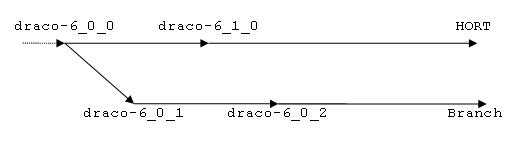
\includegraphics[width=4in]{branch-example.png}}
  \caption{Schematic of a bug-fix branch in \cvs\ .}
  \label{fig:branch}
\end{figure}

%%---------------------------------------------------------------------------%%
%% Procedures
%%---------------------------------------------------------------------------%%

\section{Draco Release Procedures}
\label{sec:procedures}

In \S~\ref{sec:policy} we have defined a set of policies that dictate
a code release process for \draco.  In this section we shall proceed
to define procedures for accomplishing those policies.  

%%---------------------------------------------------------------------------%%

\subsection{Prerequisits for Release}
\label{sec:prereq}

The following checklist provides the basic procedure that should be
followed when making a formal release of the \draco\ libraries and
binaries.
\begin{enumerate}
\item Determine what capabilities/bugs must be implemented/fixed for
  release.  This is often a list generated at a team meeting or
  through email discussions. The
  \href{http://tf.lanl.gov/sf/projects/draco}{TeamForge} {\it version}
  key on tracker artifacts can also be used to help with this item.
  This information should be recorded in the top level
  \texttt{ChangeLog}.  The format for your release notes should be
  similar to previous release notes in the \texttt{ChangeLog}.
\item Because several projects link against \draco, the release should
  be coordinated with all parties involved.  At a minimum, the
  \capsaicin\ and \jayenne\ teams should be involved with planning the
  release.
\item Ensure appropriate unit testing for each package.  All tests
  must report pass when \ctest\ is executed from the \draco\ build
  directory for each build type (e.g: \texttt{Debug} with full DbC,
  \texttt{Release} without DbC, etc.). The code coverage reports found
  on \href{http://coder.lanl.gov/cdash}{CCS--2's CDash server} may
  also be used to evaluate if additional tests are needed.
\item Ensure that the software will compile and all tests will pass
  for target platforms and build types. See the provided build script
  in \S~\ref{sec:generating_release} and
  Table~\ref{tab:supported_platforms} for details about how to compile
  \draco\ and run the tests.
\item Propose a release date.  This proposal should be send to the
  \href{mailto:draco@lanl.gov}{Draco mailing list}. 
\item Vendors: Note that you may also need to build and install vendor libraries
  at \url{/usr/projects/draco/vendors} (i.e.: atlas, gsl, etc.).  See
  \S~\ref{sec:vendors} for more details. 
\end{enumerate}
With the above items complete, the release process can begin.

%%---------------------------------------------------------------------------%%

\subsection{Identify the Last Release}
\label{sec:last_rel}

The last release can be identified in a number of ways.  Start by
examining the \texttt{ChangeLog}, the version numbers found in
\texttt{CMakeLists.txt}, release notes and email notification from
prior releases.  However, this process will rely primary on the
\cvs\ tag values for the top level \texttt{CMakeLists.txt}.

Ensure that the working copy of draco is at the \texttt{HEAD} of the
\cvs\ repository by executing the command '\texttt{cvs -q update
  -AdP}' from the \draco\ source directory.  Now examine the \cvs\ log
for \texttt{CMakeLists.txt} as follows:
%
\lstset{language=ksh,
  showstringspaces=false,
  frame=shadowbox,
  basicstyle=\footnotesize,
  rulesepcolor=\color{black},
  backgroundcolor=\color{listingBG}
}
\begin{lstlisting}[basicstyle=\footnotesize, xleftmargin=1.0in, 
  xrightmargin=1.0in]
cd draco
cvs log CMakeLists.txt | more

   RCS file: /ccs/codes/radtran/cvsroot/draco/CMakeLists.txt,v
   Working file: CMakeLists.txt
   head: 1.31
   symbolic names:
        draco-6_3_0: 1.31
        draco-6_2_1: 1.27
        draco-6_2_0: 1.25
        draco-6_1_0: 1.18
        draco-6_0_0: 1.9
        draco-5_21_0: 1.5
...
\end{lstlisting}
%
Take note of the list of {\it symbolic links}.  The largest value
should correspond to the most recent \draco\ release.  In the example
above, the most recent release was \texttt{draco-6\_3\_0}.  If the
next release is a major release, its version tag will be
\texttt{draco-7\_0\_0}.  If the next release is a minor release, the
version tag will be \texttt{draco-6\_4\_0} and if the next release is
a bug fix or patch release it will be named \texttt{draco-6\_3\_1}.

%%---------------------------------------------------------------------------%%

\subsection{Generate ChangeLog}
\label{sec:changelog}

The \texttt{ChangeLog} is a text file in the source tree that provides
a summary of the release.  See \S~\ref{sec:policy} for a list of items
that must be included in the \texttt{ChangeLog} for each release.
Often it is desireable to cut and paste previous release notes from
the \texttt{ChangeLog}.  The {\it release coordinator} should generate
the release entry in the \texttt{ChangeLog}.

The first line of release entry should be the proposed release version
and specify in text if this is a {\it major}, {\it minor} or {\it
  patch} release.  The type of release must be decided by the
\draco\ board based on the number and significance of proposed
changes.

The second entry should list the supported platforms, compilers and
vendors for the release.  This is usually specified by the customer.

%%---------------------------------------------------------------------------%%

\subsubsection{Target Platforms}
\label{sec:target_platforms}

\draco\ is used by the Eularian Applications Project, EAP, and the
target platforms for each release will mirror EAP's targets.  The best
way to determine the target platforms and the compiler and vendor
versions for each platform is to examine EAP's configuration file
\url{/usr/projects/crestone/dotfiles/Cshrc}.  Currently, the machines
and compiler sets listed in Table~\ref{tab:supported_platforms} are
supported.
%
\begin{table}[ht]
  \caption{Supported Platforms and Compilers for Draco Releases}
  \label{tab:supported_platforms}
\begin{center}
\begin{tabular}{lll} \hline\hline
\multicolumn{1}{c}{Machine} & 
\multicolumn{1}{c}{Compiler Set} & 
\multicolumn{1}{c}{Vendors} \\ \hline
TLCC hurricane/turing & Intel 10.0.023 &  OpenMPI-1.4.3 \\
                      & PGI 9.0-3      &  OpenMPI-1.4.3 \\
Roadrunner/rr\_dev    & GCC 4.3.0      &  OpenMPI-1.4.3 \\
YellowRail            & PGI 9.0-3      &  OpenMPI-1.4.3 \\
Dawn                  & --             &  --             \\
Ceilo/Ceilito         & PGI 10.9.0     &  MPICH2-5.2.0.7 \\
Moonlight             & --             & --             \\
Mapache               & --             & --             \\
\hline\hline
\end{tabular}
\end{center}
\end{table}

Development is primary done on CCS--2 LAN machines such as
\texttt{ccscs8}, \texttt{ccscs9} and on personal RedHat Linux and
Macintosh OS/X workstations.  These platforms are informally supported
with various compiler (GNU, Portland Group, Intel) and vendor sets.  

%%---------------------------------------------------------------------------%%

\subsubsection{Identify and record changes since last release}
\label{sec:changes_since_lr}

A summary changes per component will be included in the
\texttt{ChangeLog}, including changes to the build system,
\draco\ developer environment and documents. It is unfortunate that
\cvs\ records change information per file instead of by commit because
it makes it a bit painful to extract information changes since the
last release.  Here is the process that can provide this information.

\begin{enumerate}
\item Generate a list of files that have been modified since the last
  release and count the files.
\begin{lstlisting}[basicstyle=\footnotesize, xleftmargin=1.0in, 
  xrightmargin=1.0in]
cvs -q diff -N -c -r draco-6_3_0 | grep "Index: " > files_changed.log
num_files_changed=`cat files_changed.log | sort -u | wc -l`
echo $num_files_changed
\end{lstlisting}
%$
\item Generate a log file that contains all changes since the last
  release.  This command doesn't work with symbolic tag names and you
  must use a date range instead.  The date of the last release can be
  taken from the \texttt{ChangeLog}.
\begin{lstlisting}[basicstyle=\footnotesize, xleftmargin=1.0in, 
  xrightmargin=1.0in]
cvs -q log -NS -d"2011-01-06<now" > comments_since_last_release.log
\end{lstlisting}
% -N don't print a list of tags
% -S suppress the header
\item The total number of commits since the last release can be
  aproximated using the following script:
\begin{lstlisting}[basicstyle=\footnotesize, xleftmargin=1.0in, 
  xrightmargin=1.0in]
grep "date: "  comments_since_last_release.log | \
     sed -e 's/state.*//g' | sort -u | wc -l
\end{lstlisting}
\item Go through the file \texttt{comments\_since\_last\_release.log}
  and summarize the log entries in the \texttt{ChangeLog}.
\end{enumerate}

Record the number of files modified and the number of commits to the
\texttt{ChangeLog}. Summarize the \cvs\ commit messages per component.
If a \cvs\ commit message is confusing or incomplete the release
coordinator should contact the author to clarify the change.

%%---------------------------------------------------------------------------%%

\subsubsection{Generate a list of known and corrected defects}
\label{sec:list_of_defects}

\draco\ uses the \href{https://tf.lanl.gov}{LANL TeamForge server} for
tracking defects.  A list of known defects can be copied directly from
the \texttt{Tracker::Bugs} summary page.  A snapshot of this defect
list is shown in Figure~\ref{fig:sample-bug-itemization-on-tf}. At
this time it is useful to go through the bugs listed in the tracker
and provide updates as needed.  This is a good opportunity to remind
developers of defects they are assigned to.  Note that all
\textit{Priority 1} defects must be resolved before the release can
continue.

\begin{figure}
  \centerline{ 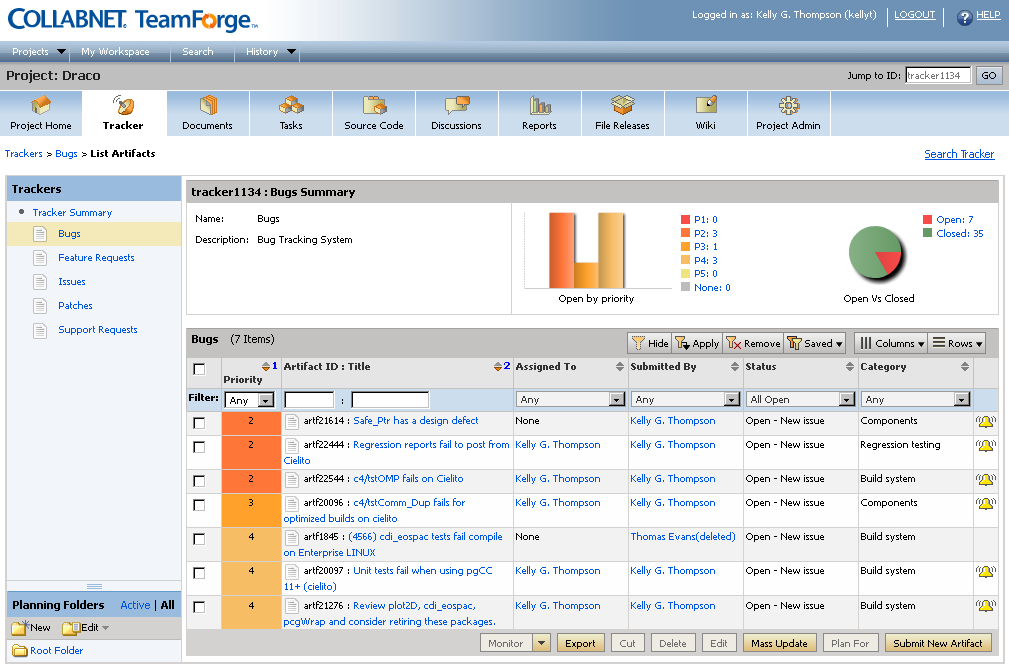
\includegraphics[height=5.25in, angle=90]
{sample-bug-itemization-on-tf.png}}
  \caption{A list of active defects for \draco\ is maintained on
    LANL's TeamForge server.  This list can be copied directly into
    the \texttt{ChangeLog}.}
  \label{fig:sample-bug-itemization-on-tf}
\end{figure}

Resolved defects are also extracted from the \draco\ page on
TeamForge.  You will need to navigate to the \texttt{Reports} tab and
then select and edit the report for \texttt{Recently closed bugs}.
Update the date range for \textit{Closed} to match the date of the
previous release up to the current date and then generate the report
by selecting the \textit{Report Details} tab as shown in
Figure~\ref{fig:sample-resolved-defect-list}.  The list of resolved
defects can be copied to \texttt{ChangeLog}.

\begin{figure}
  \centerline{ 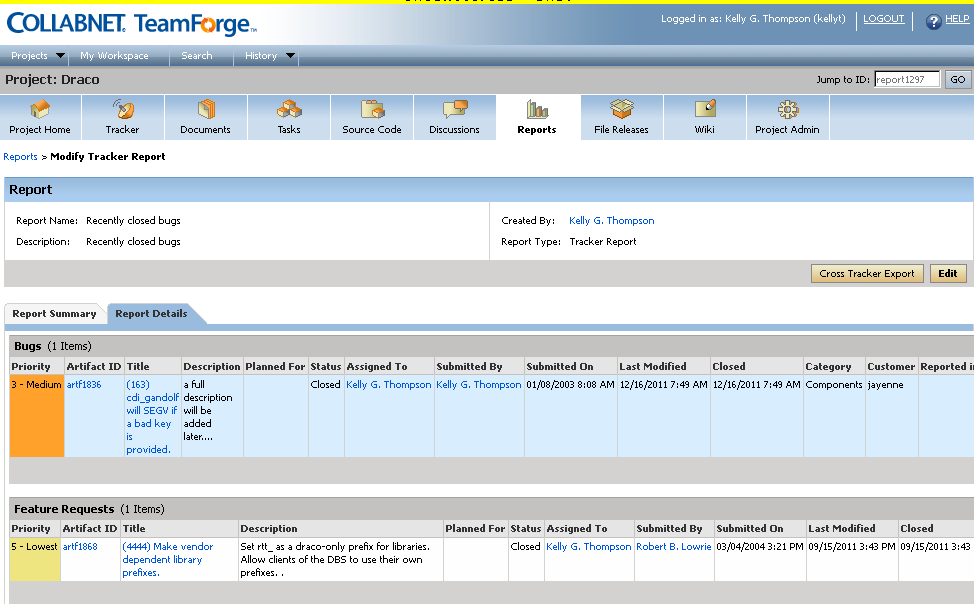
\includegraphics[height=5.0in, angle=90]
{sample-resolved-defect-list.png}}
  \caption{A list of resolved defects for \draco\ is reported by
    LANL's TeamForge server.  This list can be copied directly into
    the \texttt{ChangeLog}.}
  \label{fig:sample-resolved-defect-list}
\end{figure}

%%---------------------------------------------------------------------------%%

\subsubsection{Code Metrics}
\label{sec:code_metric}

The last set of data required for the release note in the
\texttt{ChangeLog} are the current code statistics including total
lines-of-code, LOC, as reported by the \draco\ tool
\texttt{count\_loc.sh} and the function point code coverage as
reported by the Bullseye tool~\cite{bullseyeweb}.

The LOC metric is generated by running the \draco\ tool
\texttt{count\_loc.sh} from the \draco\ source directory.  This report
can be copied directly into the \texttt{ChangeLog}.
%
\begin{lstlisting}[basicstyle=\footnotesize, xleftmargin=1.0in, 
  xrightmargin=1.0in]
cd draco
tools/count_loc.sh

Counting lines of source code --
Directory:  /home/kellyt/draco
Date     :  Mon Jan 9 10:13:18 MST 2012

                 Total C++ source: 40418
   C++ source in test directories: 22788
      C++ contract specifications: 1549
                     C++ comments: 42466
             Total Fortran source: 0
                 Fortran comments: 0
              LaTeX Documentation: 15427
                      HTML source: 0
                        Text docs: 7589
       Build system script source: 9958
   Executable shell script source: 599
           Executable Perl source: 1867
                    Python source: 3870
                    Expect source: 0
                     Elisp source: 6696
\end{lstlisting}

The code coverage data can be extracted from the coverage data file
that is generated during the nightly regression test on
\texttt{ccscs8}. This report can be copied directly into the
\texttt{ChangeLog}. 
%
\begin{lstlisting}[basicstyle=\footnotesize, xleftmargin=1.0in, 
  xrightmargin=1.0in]
cd /home/regress/cmake_draco/Nightly_gcc/Coverage/build
export COVFILE=`pwd`/CMake.cov
export COVDIRCFG=`pwd`/covclass_cmake.cfg
cd ../source/src; covdir -p

Directory               Function Coverage           C/D Coverage
------------------  ---------------------  ---------------------
units/                  82 /    82 = 100%      58 /    58 = 100%
traits/                 16 /    16 = 100%       0 /     0
diagnostics/             8 /     8 = 100%       4 /     4 = 100%
special_functions/      29 /    29 = 100%     190 /   198 =  95%
fit/                     1 /     1 = 100%      15 /    16 =  93%
ode/                     5 /     5 = 100%      29 /    32 =  90%
cdi/                    39 /    39 = 100%      27 /    30 =  90%
min/                     9 /     9 = 100%     137 /   154 =  88%
linear/                 16 /    16 = 100%     324 /   392 =  82%
roots/                   8 /     8 = 100%     256 /   312 =  82%
mesh_element/           24 /    24 = 100%     165 /   213 =  77%
cdi_ipcress/           106 /   106 = 100%     191 /   252 =  75%
meshReaders/            15 /    15 = 100%     127 /   172 =  73%
fpe_trap/                2 /     2 = 100%       4 /    11 =  36%
RTT_Format_Reader/     315 /   321 =  98%     273 /   356 =  76%
ds++/                  632 /   651 =  97%     571 /   643 =  88%
norms/                  25 /    26 =  96%      21 /    34 =  61%
viz/                    24 /    25 =  96%     129 /   168 =  76%
timestep/               59 /    62 =  95%     104 /   178 =  58%
c4/                    177 /   189 =  93%     352 /   406 =  86%
cdi_analytic/          130 /   140 =  92%     156 /   190 =  82%
rng/                    62 /    67 =  92%      63 /    70 =  90%
parser/                246 /   266 =  92%    1050 /  1351 =  77%
quadrature/            167 /   188 =  88%     517 /   683 =  75%
plot2D/                 22 /    29 =  75%      46 /    76 =  60%
lapack_wrap/            11 /    16 =  68%       0 /     0
------------------  ---------------------  ---------------------
Total                 2230 /  2340 =  95%    4809 /  5999 =  80%
\end{lstlisting}

%%---------------------------------------------------------------------------%%

\subsection{Update the version tags}
\label{sec:update_tags}

Now that the \texttt{ChangeLog} is complete, it is time to update the
version information in the code and tag the \cvs\ repository.  The
version number as reported by \textsf{ds++}'s \texttt{Release()}
function is recorded in the code at \texttt{CMakeLists.txt}.  Update
the following two lines and commit the file to \cvs.
%
\begin{lstlisting}[basicstyle=\footnotesize, xleftmargin=2.0in, 
  xrightmargin=2.0in]
#
# The Draco version number.
#
set(DRACO_VERSION_MAJOR 6)
set(DRACO_VERSION_MINOR 3)
\end{lstlisting}
% 
The value of \texttt{DRACO\_VERSION\_PATCH} is set manually during a
release build.  For development builds the third portion of the
version tag will be set to the configure date (e.g.:
\texttt{draco-6\_3\_20120113} for code configured on January 13,
2012).  Note that the version tag is stored in the file
\texttt{ds++/config.h} and can be extracted with the command
\begin{lstlisting}[basicstyle=\footnotesize, xleftmargin=2.0in, 
  xrightmargin=2.0in]
grep DRACO_VERSION_FULL ds++/config.h 
\end{lstlisting}

It may be necessary to update the version name in
\texttt{README.draco} and in other documents found in the source
repository.  Use your discretion to determine what documents need to
be updated.  For the \texttt{README.draco} file, the author list may
needed to be updated.

Before tagging the \cvs\ repository, ensure that all changes in your
local copy are checked in.  This is often done with a command similar
to
%
\begin{lstlisting}[basicstyle=\footnotesize, xleftmargin=1.0in, 
  xrightmargin=1.0in]
cvs commit -m"Preparing for the release of draco-6_4_0"
cvs -nq update 
\end{lstlisting}
%
Assuming that the working directory is fully sychronized with the HEAD
revision of the \cvs\ repository, we can tag the release.
%
\begin{lstlisting}[basicstyle=\footnotesize, xleftmargin=2.0in, 
  xrightmargin=2.0in]
cvs tag 'draco-6_4_0'
\end{lstlisting}

\subsubsection{Moving a tag}
If a file needs to be updated later in the release process, the
symbolic tag can be moved on a file by file basis using a command
similar to
%
\begin{lstlisting}[basicstyle=\footnotesize, xleftmargin=2.0in, 
  xrightmargin=2.0in]
cvs tag -r 1.6 -F draco-6_4_0 myfile.cc
\end{lstlisting}
% 
In this example, the `1.6` is the current version of the modified file
as reported by '\texttt{cvs log myfile.cc}.'

\subsubsection{Major \cvs\ tag numbers}
When producing a \textit{major} release, the first digit of the
\cvs\ tag should also be moved. This can be accomplished as follows
%
\begin{lstlisting}[basicstyle=\footnotesize, xleftmargin=2.0in, 
  xrightmargin=2.0in]
cvs commit -r 6.0
\end{lstlisting}
%
This command will commit any changes to the source and will update the
revision numbers of all files to '6.0.'  This step should precede the
tagging command.

\subsubsection{Bug Fixes}

As mentioned in the policy section, bug fixes are handled on
\cvs\ branches.  To generate such a branch the following
\cvs\ commands are used:
\begin{lstlisting}[basicstyle=\footnotesize, xleftmargin=2.0in, 
  xrightmargin=2.0in]
cvs -q checkout -r draco-1_4_0 draco
cvs tag -b draco-1_4_1
\end{lstlisting}
This creates a branch to \draco\ release~1.4.  If the bug fix is
required in a \draco\ release, \draco\ should be re-released with the
appropriate branch number.  Branches are used for bug fixes only.

Additional fixes of bugs on this branch should be tagged using
\texttt{cvs tag draco-1\_9\_2}.  Thus, to make a tag to this version
use the following commands:
\begin{lstlisting}[basicstyle=\footnotesize, xleftmargin=2.0in, 
  xrightmargin=2.0in]
cvs checkout -r draco-1_4_1 draco
(make changes)
(run regression tests)
cvs tag draco-1_4_2
\end{lstlisting}
We note that \cvs\  branches automatically release code to the end
of the branch.  Hence, \texttt{cvs checkout -r draco-1\_4\_1 draco}
will automatically give the sources at the end of the \draco\ branch
connected to release~1.4.  We add tags to clarify the development and
bug tracking process in \draco\ even though they may not be strictly
necessary in all cases.  For more information on branches, see
Chapter~5 of the \cvs\  manual.

%%---------------------------------------------------------------------------%%

\subsection{Generating the release}
\label{sec:generating_release}

Releases are only generated on HPC hardware (Turing, Cielito, etc.).
Because of software environment changes, this set of instruction is
only a guide and may need to be modified slightly based on each
situation. The steps for generating a release are: creating the
release file structure, setting the software environment, obtained the
source code, building, testing and installing the product, and
checking for errors or warnings.
%
\begin{enumerate}
\item Create the install location by following the example of previous
  releases.  Create a release directory structure based on the version
  name.
\begin{lstlisting}[basicstyle=\footnotesize, xleftmargin=0.20in, 
  xrightmargin=0.20in]
mkdir -p /usr/projects/draco/draco-6_3_0/source
mkdir -p /usr/projects/draco/draco-6_3_0/logs
cp -r /usr/projects/draco/draco-6_2_0/scripts /usr/projects/draco/draco-6_3_0/scripts
\end{lstlisting}
\item Access the tagged source code.
\begin{lstlisting}[basicstyle=\footnotesize, xleftmargin=1.0in, 
  xrightmargin=1.00in]
cd /usr/projects/draco/draco-6_3_0/source
export CVS_RSH=ssh
export CVSROOT=ccscs8:/ccs/codes/radtran/cvsroot
cvs -q co -P -r draco-6_3_0 draco
\end{lstlisting}
\item Edit the build/test/release scripts found at
  \url{/usr/projects/draco/draco-6_3_0/scripts}. 
\item Review the customer's desired compiler set for this platform.
  This can be accomplished by reviewing or sourcing
  \url{/usr/projects/crestone/dotfiles/Cshrc}.  These changes should
  be added to the build/test/release scripts.
\item Update the developer environment (e.g.:
  Modules~\cite{modulecmd}, vendor setups, environment variables) with
  \draco\ specific settings.  These changes should be added to the
  build/test/release scripts.
\item Run the build/test/release script. This script ususally builds
  several versions (debug, opt, opt non-reproducible, etc) of the code
  for one platform.  The script may be either a shell script or a
  \texttt{msub} script for submission under Torque.
\item Once the script completes, check the log file to ensure that no
  errors occured and that all tests pass.
\item A separate script must be run and the log file examined for each
  supported platform and compiler set as listed in
  Table~\ref{tab:supported_platforms}
\end{enumerate}
%
An sample release script is shown below.  This script should be edited
carefully before it is run to ensure that version numbers, locations,
build types and build environment are correctly set
%
\begin{lstlisting}[basicstyle=\footnotesize, xleftmargin=0.20in, 
  xrightmargin=0.20in]
#!/bin/env bash

#MSUB -V
#MSUB -l walltime=01:00:00
#MSUB -l nodes=1:ppn=16
#MSUB -j oe
#MSUB -o /usr/projects/draco/draco-6_3_0/logs/release_tu.log

#----------------------------------------------------------------------#
# The script starts here
#----------------------------------------------------------------------#

# Permissions - new files should be marked u+rwx,g+rwx,o+rx
umask 0002
build_permissions="g+rwX"
install_permissions="g+rwX,o=g-w"

# environment (use draco modules)
module () 
{
  eval `/usr/bin/modulecmd bash $*` 
}
module purge
module load hpc-tools friendly-testing python cmake
module load intel-c/10.0.023 intel-f/10.0.023 openmpi-intel/1.4.3
module load gsl/1.14-intel lapack/atlas-3.8.3-intel numdiff
module list

# This is the bug fix number.  Normally set this to zero.
CONFIG_BASE="-DDRACO_VERSION_PATCH=0"

# Define your source and build information here.

ddir="draco-6_3_0"
platform="tu"
dmpi=openmpi143
df90=gfortran
dcpp=g++

# Define or source your platform information here
dcpp=intel100023
df90=$dcpp

# Locations for source, build and install
source_prefix="/usr/projects/draco/$ddir"
build_prefix="/scratch/$USER/$ddir/$platform-${dmpi}-${df90}-${dcpp}"
install_prefix="$source_prefix/$platform-${dmpi}-${df90}-${dcpp}"

# Helpful functions:
die () { echo "ERROR: $1"; exit 1;}

run () {
    if [ $dry_run ]
    then echo $1
    else eval $1
    fi
}

# Define the meanings of various configure features:
DBC_OFF="-DDRACO_DBC_LEVEL=0"
DBC_ON="-DDRACO_DBC_LEVEL=7"

OPTIMIZE_ON="-DCMAKE_BUILD_TYPE=Release"
OPTIMIZE_OFF="-DCMAKE_BUILD_TYPE=Debug"

LOGGING_ON="-DDRACO_DIAGNOSTICS=7 -DDRACO_TIMING=1"
LOGGING_OFF="-DDRACO_DIAGNOSTICS=0 -DDRACO_TIMING=0"

NR_ON="-DENABLE_RNG_NR=ON"
NR_OFF="-DENABLE_RNG_NR=OFF"

# Define the meanings of the various code versions:
VERSIONS=(\
    "debug"    "debug_nodbc"    "opt"    "opt_log" \
    "debug_nr" "debug_nodbc_nr" "opt_nr" "opt_log_nr" \
)
OPTIONS=(\
    "$DBC_ON  $OPTIMIZE_OFF $LOGGING_ON  $NR_OFF" \
    "$DBC_OFF $OPTIMIZE_OFF $LOGGING_ON  $NR_OFF" \
    "$DBC_OFF $OPTIMIZE_ON  $LOGGING_OFF $NR_OFF" \
    "$DBC_OFF $OPTIMIZE_ON  $LOGGING_ON  $NR_OFF" \
\
    "$DBC_ON  $OPTIMIZE_OFF $LOGGING_ON  $NR_ON"  \
    "$DBC_OFF $OPTIMIZE_OFF $LOGGING_ON  $NR_ON"  \
    "$DBC_OFF $OPTIMIZE_ON  $LOGGING_OFF $NR_ON"  \
    "$DBC_OFF $OPTIMIZE_ON  $LOGGING_ON  $NR_ON"  \
)
PACKAGES=("draco")

# =============
# Configure, Build and Run the Tests
# =============


# Loop over the code versions:

for (( i=0 ; i < ${#VERSIONS[@]} ; ++i ))
do

    version=${VERSIONS[$i]}
    options=${OPTIONS[$i]}

    echo
    echo
    echo "# Code Version: $version"
    echo "# ------------"
    echo

    # Create install directory
    install_dir="$install_prefix/$version"
    run "mkdir -p $install_dir" || die "Could not create $install_dir"

    # Loop over the packages.
    for package in ${PACKAGES[@]}
    do
        echo
        echo "#    Package: $package"
        echo "#    -------"
        echo
        
        source_dir="$source_prefix/source/$package"
        build_dir="$build_prefix/$version/${package:0:1}"

        run "mkdir -p $build_dir" || die "Could not create directory $build_dir."
        run "cd $build_dir"
        run "cmake -DCMAKE_INSTALL_PREFIX=$install_dir \
            $options $CONFIG_BASE $source_dir" \
            || die "Could not configure in $build_dir from source at $source_dir"
        run "make -j20 all"  || die "Could not build code/tests in $build_dir"
        run "ctest -j16" # Allow some tests to fail.
        run "make -j20 install"  || die "Could not build code/tests in $build_dir"
        run "chmod -R $build_permissions $build_dir"

    done

    # Set access to install dir.
    run "chmod -R $install_permissions $install_dir"

done

# Set access to top level install dir.
run "chmod $install_permissions $install_prefix"
run "chgrp -R draco $install_prefix"
\end{lstlisting}
%$

%%---------------------------------------------------------------------------%%

\subsection{Release notification}
\label{sec:release_notification}

Once the release is complete, a notification via email to
\url{draco@lanl.gov} must be issued.  You may need to contact other
interested parties as well.  Sample email notices can be found in the
source repository at \url{/doc/releases}.  The notification should
also be made on TeamForge by adding the new version to the
\textit{File Releases} section and by posting a \textit{News Post}.

%%---------------------------------------------------------------------------%%

\subsection{Backup the release}
\label{sec:backup_rel}

The release must also be backed up to the tri-lab archive.  From a
CCS--2 LAN machine, tar the \cvs\ repository and copy the tar file to
\url{/usr/projects/asc\_bkups} on HPC.
\begin{lstlisting}[basicstyle=\footnotesize, xleftmargin=1.0in, 
  xrightmargin=1.00in]
# CCS-2 LAN
cd /ccs/codes/radtran/cvsroot
tar --use-compress-program /usr/bin/bzip2 -cvf draco.tar.bz2 draco
push draco.tar.bz2
# HPC
cd /usr/projects/asc_bkups/draco
pull 1 draco.tar.bz2
\end{lstlisting}

%%---------------------------------------------------------------------------%%

\subsection{Generating a contributing author list}
\label{sec:author_list}

If a contributing author list is required (i.e.: for use in a release
memo or other document), the following procedure may be used:

\begin{enumerate}
\item Generate a list of files found in this release:
\begin{lstlisting}[basicstyle=\footnotesize, xleftmargin=0.75in, 
  xrightmargin=0.75in]
files=`find . -name '*.hh' -o -name '*.cc' -o -name '*.txt' \
       -o -name '*.cmake' -o -name '*.in' -o -name '*.h'`
cvs annotate $files > file_list
\end{lstlisting}
\item Generate a list of authors.
\begin{lstlisting}[basicstyle=\footnotesize, xleftmargin=0.75in, 
  xrightmargin=0.75in]
user_list=`cat file_list | awk '{print $2}' | sort -u | sed -e 's/^(//'`
\end{lstlisting}
\item Generate a report
\begin{lstlisting}[basicstyle=\footnotesize, xleftmargin=0.75in, 
  xrightmargin=0.75in]
for name in $user_list; do numlines=`grep $name file_list | wc -l`; \
     echo "$numlines: $name"; done > author_loc
cat author_loc | sort -rn

68326: kellyt
45126: kgbudge
23521: tme
7378: lowrie
6153: bta
5541: mwbuksas
4360: mcghee
2807: pautz
2489: phenning
2368: warsa
2186: rsqrd
2005: gaber
1201: furnish
...
\end{lstlisting}
\end{enumerate}

Monikers can be converted to full names by using the \texttt{finger}
command. 

%%---------------------------------------------------------------------------%%

\section{Vendors}
\label{sec:vendors}

\draco\ depends on a few third party vendors to provide full
functionality.  These vendors are typically loaded into the developer
environment through the use of \texttt{module}
commands~\cite{modulecmd}.  Vendor libraries are loaded from the local
system if available.  Otherwise, the vendor libraries can be loaded
from either \url{/usr/projects/draco/vendors} or
\url{/ccs/codes/radtran/vendors/Linux64} through the use of
\draco\ '\texttt{module load}' commands.

Currently, \draco\ can make use of the following vendor libraries
%
\begin{table}[ht]
  \caption{Vendor libraries used by \draco}
  \label{tab:vendors}
\begin{center}
\begin{tabular}{lll} \hline\hline
% \begin{tabular}{llp{8cm}} \hline\hline
\multicolumn{1}{c}{Vendor name} & 
\multicolumn{1}{c}{Recommended Version} & 
\multicolumn{1}{c}{Required or Optional} \\ \hline
OpenMPI                & 1.3.3+ & Required \\
GNU Scientific Library & 1.14+  & Required \\
Numdiff                & 5.2.1+ & Required \\
Python                 & $<$3.0 & Required \\
CMake                  & 2.8.6+ & Required \\
LAPACK                 & 2.8.3+ & Optional \\
Grace (gnuplot)        & 4.4+   & Optional \\
PAPI                   & 4.1+   & Optional \\
\hline\hline
\end{tabular}
\end{center}
\end{table}

%%---------------------------------------------------------------------------%%

%% \section{Future Directions}
%% \label{sec:future}

%% \begin{itemize}
%% \item Move to git
%% \item Require bug tracking database
%% \item Description of code coverage and memory instrumentation
%%   requirements and tools.
%% \end{itemize}

%%---------------------------------------------------------------------------%%

\section{Summary}
\label{sec:summary}

We have detailed the release policies and procedures for
\draco\ projects in group CCS--2.  As with all \draco\ policies,
exceptions to the standard rules are acceptable pending review by
\draco\ team members.  These procedures have been reviewed and are
part of the \draco\ development process. While the basic procedures
explained in this document are robust, all procedures could benefit
from future enhancements and this document should be updated as
needed. 
%A list of
%desired improvements to the \draco\ release procedures are:
%\begin{itemize}
%\item \cvs\  major revision numbers could be updated auto-magically
%  when the major release numbers on the tag are advanced.
%\end{itemize}
%These topics are noted for future consideration.

%%---------------------------------------------------------------------------%%

\bibliographystyle{rnote}
\bibliography{draco}

\closing
\end{document}

%%---------------------------------------------------------------------------%%
%% end of draco-release.tex
%%---------------------------------------------------------------------------%%
